\documentclass[10pt]{article} 
\usepackage[a4paper, margin=2.5cm]{geometry} 
\usepackage[T1]{fontenc} 
\usepackage[utf8]{inputenc} 
\usepackage{mathpazo} 
\usepackage[spanish]{babel} 
\usepackage{graphicx}
\usepackage{xcolor}
\usepackage{amsmath}
\usepackage{mathpazo}

\title{Caracterización de cuadripolos\\Laboratorio de Teoría de Circuitos III}
\author{Oscar Perpiñán y Luis Badesa}

\begin{document}

\maketitle


\section{Definición de cuadripolo}

Un cuadripolo es un conjunto de elementos eléctricos interconectados con cuatro bornes de acceso, agrupados en dos puertos, uno de entrada y otro de salida. Un cuadripolo se emplea para modelar equipos de transmisión, filtros, o líneas de transporte de energía eléctrica, usando un rectángulo como representación para indicar que la estructura interna no es relevante. El comportamiento del cuadripolo se determina a través de las relaciones entre las tensiones y corrientes en los puertos. 
\begin{center}
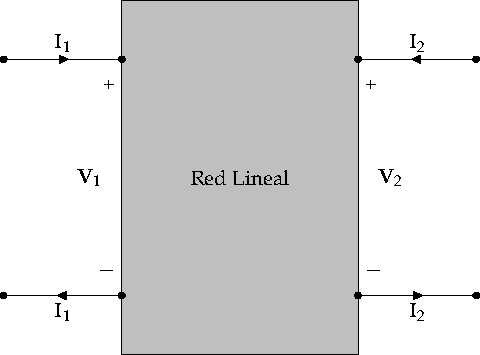
\includegraphics[height=5cm]{../figs/cuadripolo.pdf}
\end{center}

Las relaciones pueden expresarse de forma diversa, dando lugar a diferentes familias de parámetros. En este documento distinguiremos cuatro familias:
\begin{itemize}
\item Parámetros impedancia: las tensiones se expresan en función de las corrientes.
\item Parámetros admitancia: las corrientes se expresan en función de las tensiones.
\item Parámetros híbridos: la tensión de entrada y la corriente de salida se expresan en función de la tensión de salida y la corriente de entrada.
\item Parámetros híbridos inversos: la corriente de entrada y la tensión de salida se expresan en función de la tensión de entrada y la corriente de salida.
\end{itemize}

En estas relaciones es importante prestar atención al sentido de las corrientes que se muestra en la figura.

Las ecuaciones que se recogen a continuación emplean una nomenclatura genérica válida tanto para Laplace como para fasores, empleando el resaltado en negrita para tensiones, corrientes e impedancias. Los parámetros del cuadripolo se muestran en minúsculas, y las impedancias del circuito en mayúsculas.

\clearpage

\section{Caracterización de Cuadripolos}

\subsection{Parámetros de Impedancia}

\subsubsection*{Definición y circuito equivalente}


\begin{minipage}{0.5\textwidth}
\begin{center}
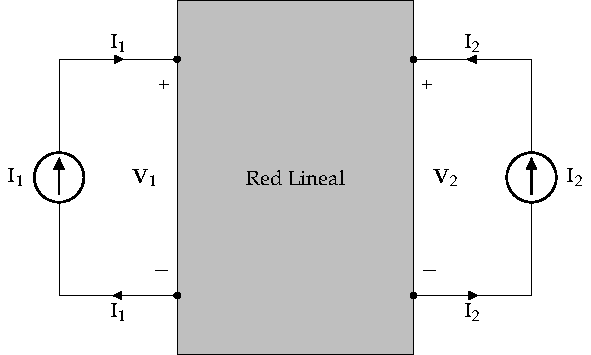
\includegraphics[height=4cm]{../figs/cuadripolo_fuentes_corriente.pdf}
\end{center}

\end{minipage}
\begin{minipage}{0.5\textwidth}
  \[
    \begin{array}{l}
      \mathbf{U}_1 = \mathbf{z}_{11} \mathbf{I}_1 + \mathbf{z}_{12} \mathbf{I}_2\\
      \mathbf{U}_2 = \mathbf{z}_{21} \mathbf{I}_1 + \mathbf{z}_{22} \mathbf{I}_2\\
    \end{array}
  \]
\[
  \left[
    \begin{array}{c}
      \mathbf{U}_1\\
      \mathbf{U}_2
    \end{array}
  \right] =
  \left[
    \begin{array}{cc}
      \mathbf{z}_{11} & \mathbf{z}_{12}\\
      \mathbf{z}_{21} & \mathbf{z}_{22}
    \end{array}
  \right] \cdot
  \left[
    \begin{array}{c}
      \mathbf{I}_1\\
      \mathbf{I}_2
    \end{array}
  \right]
\]
\end{minipage}

\begin{center}
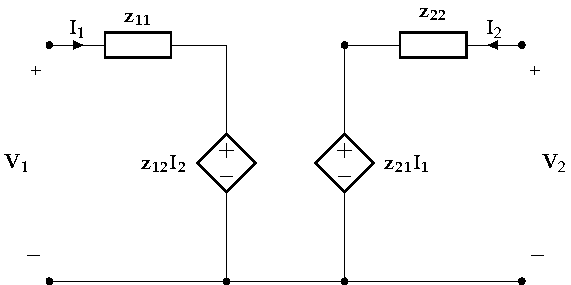
\includegraphics[height=4cm]{../figs/circuitoEquivalenteZ.pdf}
\end{center}

\subsubsection*{Medida}

\begin{minipage}{0.5\textwidth}
  \begin{center}
    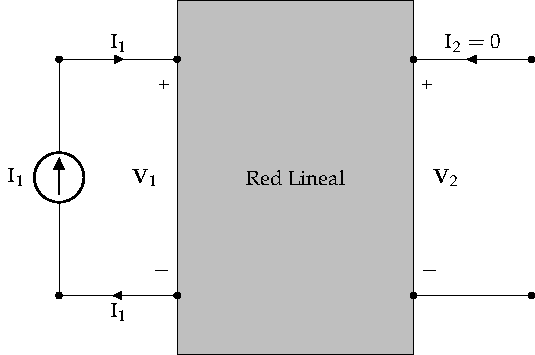
\includegraphics[height=4cm]{../figs/parametrosZ_entrada.pdf}
  \end{center}
\end{minipage}
\begin{minipage}{0.5\textwidth}
  \[
    \begin{array}{c}
      \mathbf{z}_{11} = \left.\frac{\mathbf{U}_1}{\mathbf{I}_1}\right\rvert_{\mathbf{I}_2 = 0} \\
      \mathbf{z}_{21} = \left.\frac{\mathbf{U}_2}{\mathbf{I}_1}\right\rvert_{\mathbf{I}_2 = 0}
    \end{array}
  \]

  \[
    \left[
      \begin{array}{c}
        \mathbf{U}_1\\
        \mathbf{U}_2
      \end{array}
    \right] =
    \left[
      \begin{array}{cc}
        \color{blue}{\mathbf{z}_{11}} & \mathbf{z}_{12}\\
        \color{blue}{\mathbf{z}_{21}} & \mathbf{z}_{22}
      \end{array}
    \right] \cdot
    \left[
      \begin{array}{c}
        \color{blue}{\mathbf{I}_1}\\
        \mathbf{I}_2
      \end{array}
    \right]
  \]
\end{minipage}

\vspace{1cm}

\begin{minipage}{0.5\textwidth}
  \[
    \begin{array}{c}
      \mathbf{z}_{12} = \left.\frac{\mathbf{U}_1}{\mathbf{I}_2}\right\rvert_{\mathbf{I}_1 = 0}\\
      \mathbf{z}_{22} = \left.\frac{\mathbf{U}_2}{\mathbf{I}_2}\right\rvert_{\mathbf{I}_1 = 0}
    \end{array}
  \]

  \[
    \left[
      \begin{array}{c}
        \mathbf{U}_1\\
        \mathbf{U}_2
      \end{array}
    \right] =
    \left[
      \begin{array}{cc}
        \mathbf{z}_{11} & \color{blue}{\mathbf{z}_{12}}\\
        \mathbf{z}_{21} & \color{blue}{\mathbf{z}_{22}}
      \end{array}
    \right] \cdot
    \left[
      \begin{array}{c}
        \mathbf{I}_1\\
        \color{blue}{\mathbf{I}_2}
      \end{array}
    \right]
  \]
\end{minipage}
\begin{minipage}{0.5\textwidth}
  \begin{center}
    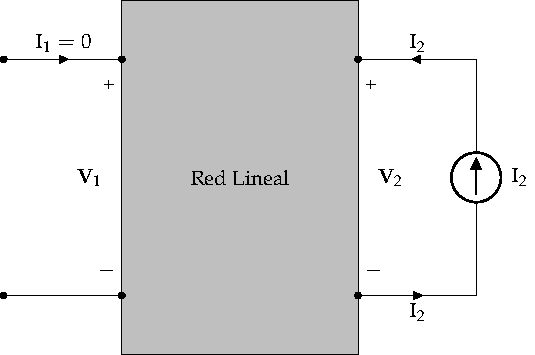
\includegraphics[height=4cm]{../figs/parametrosZ_salida.pdf}
  \end{center}
\end{minipage}

\clearpage

\subsection{Parámetros de Admitancia}

\subsubsection*{Definición y circuito equivalente}

\begin{minipage}{0.5\textwidth}
  \begin{center}
    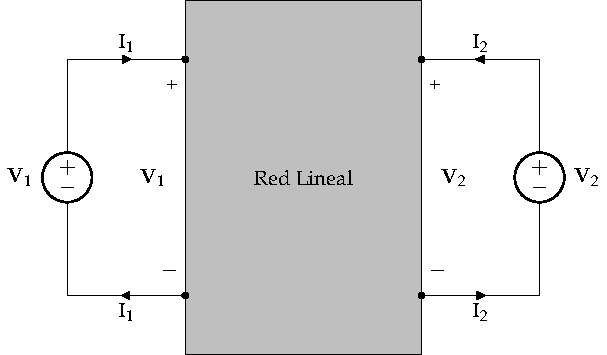
\includegraphics[height=4cm]{../figs/cuadripolo_fuentes_tension.pdf}
  \end{center}
\end{minipage}
\begin{minipage}{0.5\textwidth}
  \[
    \begin{array}{l}
      \mathbf{I}_1 = \mathbf{y}_{11} \mathbf{U}_1 + \mathbf{y}_{12} \mathbf{U}_2\\
      \mathbf{I}_2 = \mathbf{y}_{21} \mathbf{U}_1 + \mathbf{y}_{22} \mathbf{U}_2\\
    \end{array}
  \]

  \[
    \left[
      \begin{array}{c}
        \mathbf{I}_1\\
        \mathbf{I}_2
      \end{array}
    \right] =
    \left[
      \begin{array}{cc}
        \mathbf{y}_{11} & \mathbf{y}_{12}\\
        \mathbf{y}_{21} & \mathbf{y}_{22}
      \end{array}
    \right] \cdot
    \left[
      \begin{array}{c}
        \mathbf{U}_1\\
        \mathbf{U}_2
      \end{array}
    \right]
  \]
\end{minipage}

\begin{center}
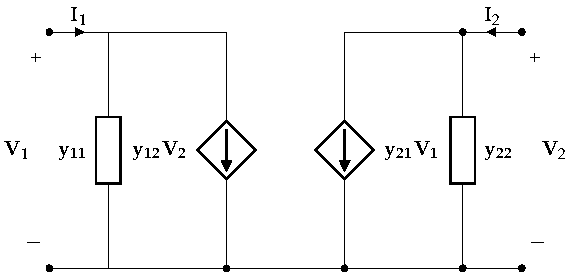
\includegraphics[height=4cm]{../figs/circuitoEquivalenteY.pdf}
\end{center}


\subsubsection*{Medida}

\begin{minipage}{0.5\textwidth}
  \begin{center}
    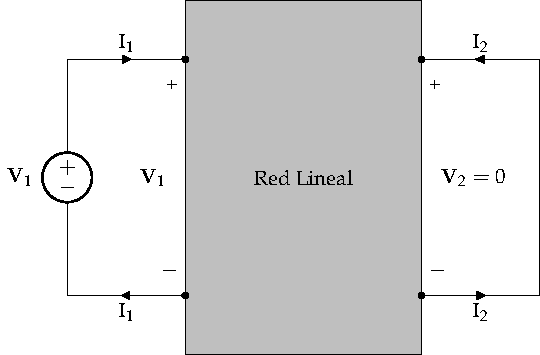
\includegraphics[height=4cm]{../figs/parametrosY_entrada.pdf}
  \end{center}
\end{minipage}
\begin{minipage}{0.5\textwidth}
  \[
    \begin{array}{c}
      \mathbf{y}_{11} = \left.\frac{\mathbf{I}_1}{\mathbf{U}_1}\right\rvert_{\mathbf{U}_2 = 0} \\
      \mathbf{y}_{21} = \left.\frac{\mathbf{I}_2}{\mathbf{U}_1}\right\rvert_{\mathbf{U}_2 = 0}
    \end{array}
  \]

  \[
    \left[
      \begin{array}{c}
        \mathbf{I}_1\\
        \mathbf{I}_2
      \end{array}
    \right] =
    \left[
      \begin{array}{cc}
        \color{blue}{\mathbf{y}_{11}} & \mathbf{y}_{12}\\
        \color{blue}{\mathbf{y}_{21}} & \mathbf{y}_{22}
      \end{array}
    \right] \cdot
    \left[
      \begin{array}{c}
        \color{blue}{\mathbf{U}_1}\\
        \mathbf{U}_2
      \end{array}
    \right]
  \]
\end{minipage}

\vspace{1cm}

\begin{minipage}{0.5\textwidth}
  \[
    \begin{array}{c}
      \mathbf{y}_{12} = \left.\frac{\mathbf{I}_1}{\mathbf{U}_2}\right\rvert_{\mathbf{U}_1 = 0}\\
      \mathbf{y}_{22} = \left.\frac{\mathbf{I}_2}{\mathbf{U}_2}\right\rvert_{\mathbf{U}_1 = 0}
    \end{array}
  \]

  \[
    \left[
      \begin{array}{c}
        \mathbf{I}_1\\
        \mathbf{I}_2
      \end{array}
    \right] =
    \left[
      \begin{array}{cc}
        \mathbf{y}_{11} & \color{blue}{\mathbf{y}_{12}}\\
        \mathbf{y}_{21} & \color{blue}{\mathbf{y}_{22}}
      \end{array}
    \right] \cdot
    \left[
      \begin{array}{c}
        \mathbf{U}_1\\
        \color{blue}{\mathbf{U}_2}
      \end{array}
    \right]
  \]
\end{minipage}
\begin{minipage}{0.5\textwidth}
  \begin{center}
    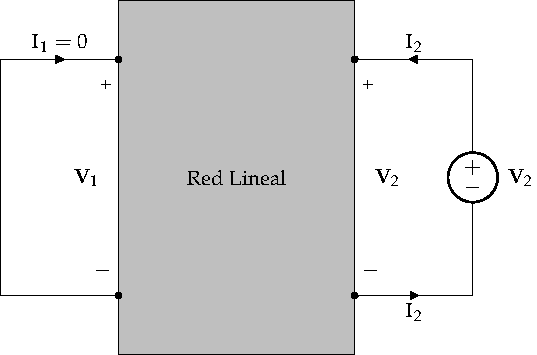
\includegraphics[height=4cm]{../figs/parametrosY_salida.pdf}
  \end{center}
\end{minipage}

\clearpage

\subsection{Parámetros Híbridos}

\subsubsection*{Definición y circuito equivalente}


\begin{minipage}{0.5\textwidth}
  \begin{center}
    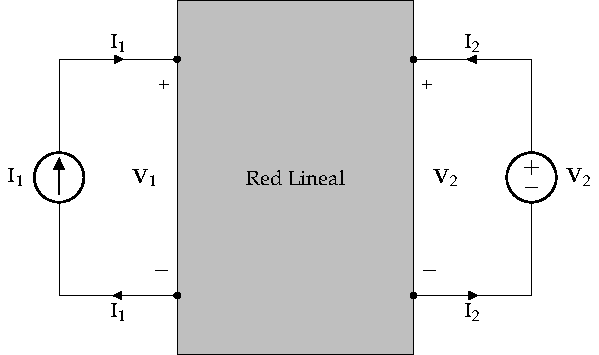
\includegraphics[height=4cm]{../figs/cuadripolo_hibrido.pdf}
  \end{center}
\end{minipage}
\begin{minipage}{0.5\textwidth}
  \[
    \begin{array}{l}
      \mathbf{U}_1 = \mathbf{h}_{11} \mathbf{I}_1 + \mathbf{h}_{12} \mathbf{U}_2\\
      \mathbf{I}_2 = \mathbf{h}_{21} \mathbf{I}_1 + \mathbf{h}_{22} \mathbf{U}_2\\
    \end{array}
  \]

  \[
    \left[
      \begin{array}{c}
        \mathbf{U}_1\\
        \mathbf{I}_2
      \end{array}
    \right] =
    \left[
      \begin{array}{cc}
        \mathbf{h}_{11} & \mathbf{h}_{12}\\
        \mathbf{h}_{21} & \mathbf{h}_{22}
      \end{array}
    \right] \cdot
    \left[
      \begin{array}{c}
        \mathbf{I}_1\\
        \mathbf{U}_2
      \end{array}
    \right]
  \]
\end{minipage}

\begin{center}
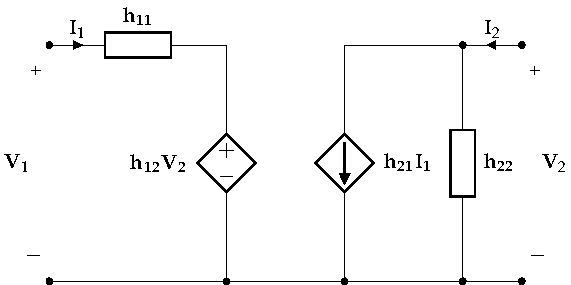
\includegraphics[height=4cm]{../figs/circuitoEquivalenteH.pdf}
\end{center}

\subsubsection*{Medida}

\begin{minipage}{0.5\textwidth}
  \begin{center}
    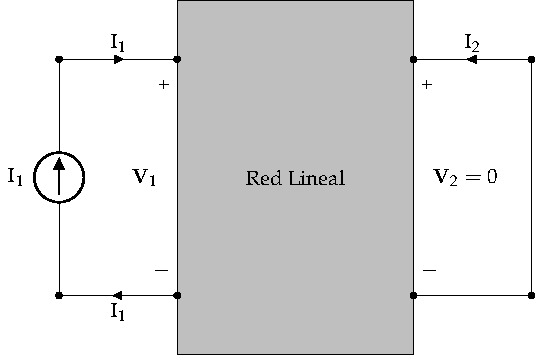
\includegraphics[height=4cm]{../figs/parametrosH_entrada.pdf}
  \end{center}
\end{minipage}
\begin{minipage}{0.5\textwidth}
  \[
    \begin{array}{c}
      \mathbf{h}_{11} = \left.\frac{\mathbf{U}_1}{\mathbf{I}_1}\right\rvert_{\mathbf{U}_2 = 0} \\
      \mathbf{h}_{21} = \left.\frac{\mathbf{I}_2}{\mathbf{I}_1}\right\rvert_{\mathbf{U}_2 = 0}
    \end{array}
  \]

  \[
    \left[
      \begin{array}{c}
        \mathbf{U}_1\\
        \mathbf{I}_2
      \end{array}
    \right] =
    \left[
      \begin{array}{cc}
        \color{blue}{\mathbf{h}_{11}} & \mathbf{h}_{12}\\
        \color{blue}{\mathbf{h}_{21}} & \mathbf{h}_{22}
      \end{array}
    \right] \cdot
    \left[
      \begin{array}{c}
        \color{blue}{\mathbf{I}_1}\\
        \mathbf{U}_2
      \end{array}
    \right]
  \]
\end{minipage}

\vspace{1cm}

\begin{minipage}{0.5\textwidth}
  \[
    \begin{array}{c}
      \mathbf{h}_{12} = \left.\frac{\mathbf{U}_1}{\mathbf{U}_2}\right\rvert_{\mathbf{I}_1 = 0}\\
      \mathbf{h}_{22} = \left.\frac{\mathbf{I}_2}{\mathbf{U}_2}\right\rvert_{\mathbf{I}_1 = 0}
    \end{array}
  \]

  \[
    \left[
      \begin{array}{c}
        \mathbf{U}_1\\
        \mathbf{I}_2
      \end{array}
    \right] =
    \left[
      \begin{array}{cc}
        \mathbf{h}_{11} & \color{blue}{\mathbf{h}_{12}}\\
        \mathbf{h}_{21} & \color{blue}{\mathbf{h}_{22}}
      \end{array}
    \right] \cdot
    \left[
      \begin{array}{c}
        \mathbf{I}_1\\
        \color{blue}{\mathbf{U}_2}
      \end{array}
    \right]
  \]
\end{minipage}
\begin{minipage}{0.5\textwidth}
  \begin{center}
    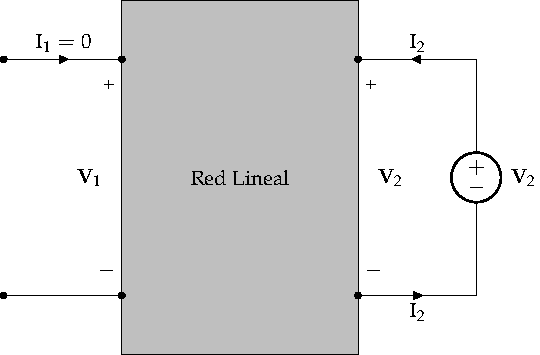
\includegraphics[height=4cm]{../figs/parametrosH_salida.pdf}
  \end{center}
\end{minipage}

\clearpage

\subsection{Parámetros Híbridos Inversos}

\subsubsection*{Definición y circuito equivalente}

\begin{minipage}{0.5\textwidth}
  \begin{center}
    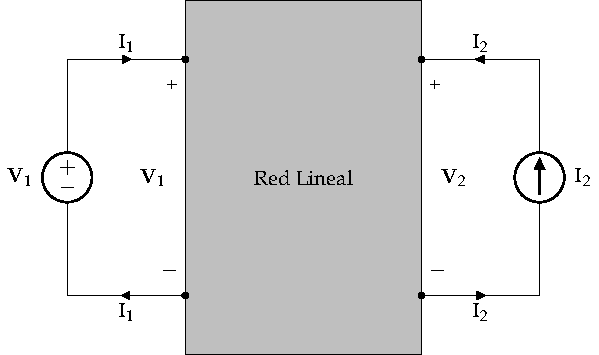
\includegraphics[height=4cm]{../figs/cuadripolo_hibrido_inverso.pdf}
  \end{center}
\end{minipage}
\begin{minipage}{0.5\textwidth}
  \[
    \begin{array}{l}
      \mathbf{I}_1 = \mathbf{g}_{11} \mathbf{U}_1 + \mathbf{g}_{12} \mathbf{I}_2\\
      \mathbf{U}_2 = \mathbf{g}_{21} \mathbf{U}_1 + \mathbf{g}_{22} \mathbf{I}_2\\
    \end{array}
  \]


  \[
    \left[
      \begin{array}{c}
        \mathbf{I}_1\\
        \mathbf{U}_2
      \end{array}
    \right] =
    \left[
      \begin{array}{cc}
        \mathbf{g}_{11} & \mathbf{g}_{12}\\
        \mathbf{g}_{21} & \mathbf{g}_{22}
      \end{array}
    \right] \cdot
    \left[
      \begin{array}{c}
        \mathbf{U}_1\\
        \mathbf{I}_2
      \end{array}
    \right]
  \]
\end{minipage}

\begin{center}
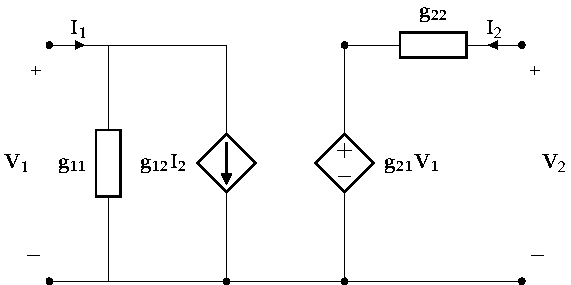
\includegraphics[height=4cm]{../figs/circuitoEquivalenteG.pdf}
\end{center}

\subsubsection*{Medida}

\begin{minipage}{0.5\textwidth}
  \begin{center}
    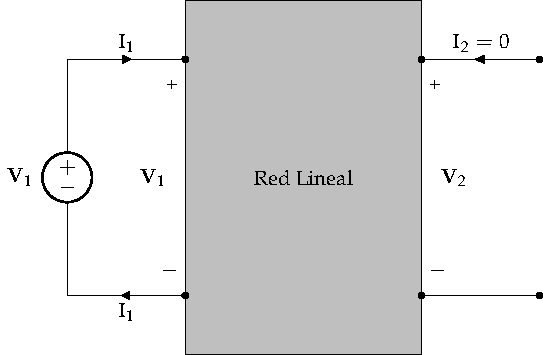
\includegraphics[height=4cm]{../figs/parametrosG_entrada.pdf}
  \end{center}
\end{minipage}
\begin{minipage}{0.5\textwidth}
  \[
    \begin{array}{c}
      \mathbf{g}_{11} = \left.\frac{\mathbf{I}_1}{\mathbf{U}_1}\right\rvert_{\mathbf{I}_2 = 0} \\
      \mathbf{g}_{21} = \left.\frac{\mathbf{U}_2}{\mathbf{U}_1}\right\rvert_{\mathbf{I}_2 = 0}
    \end{array}
  \]



  \[
    \left[
      \begin{array}{c}
        \mathbf{I}_1\\
        \mathbf{U}_2
      \end{array}
    \right] =
    \left[
      \begin{array}{cc}
        \color{blue}{\mathbf{g}_{11}} & \mathbf{g}_{12}\\
        \color{blue}{\mathbf{g}_{21}} & \mathbf{g}_{22}
      \end{array}
    \right] \cdot
    \left[
      \begin{array}{c}
        \color{blue}{\mathbf{U}_1}\\
        \mathbf{I}_2
      \end{array}
    \right]
  \]
\end{minipage}

\vspace{1cm}

\begin{minipage}{0.5\textwidth}
  \[
    \begin{array}{c}
      \mathbf{g}_{12} = \left.\frac{\mathbf{I}_1}{\mathbf{I}_2}\right\rvert_{\mathbf{U}_1 = 0}\\
      \mathbf{g}_{22} = \left.\frac{\mathbf{U}_2}{\mathbf{I}_2}\right\rvert_{\mathbf{U}_1 = 0}
    \end{array}
  \]

  \[
    \left[
      \begin{array}{c}
        \mathbf{I}_1\\
        \mathbf{U}_2
      \end{array}
    \right] =
    \left[
      \begin{array}{cc}
        \mathbf{g}_{11} & \color{blue}{\mathbf{g}_{12}}\\
        \mathbf{g}_{21} & \color{blue}{\mathbf{g}_{22}}
      \end{array}
    \right] \cdot
    \left[
      \begin{array}{c}
        \mathbf{U}_1\\
        \color{blue}{\mathbf{I}_2}
      \end{array}
    \right]
  \]
\end{minipage}
\begin{minipage}{0.5\textwidth}
  \begin{center}
    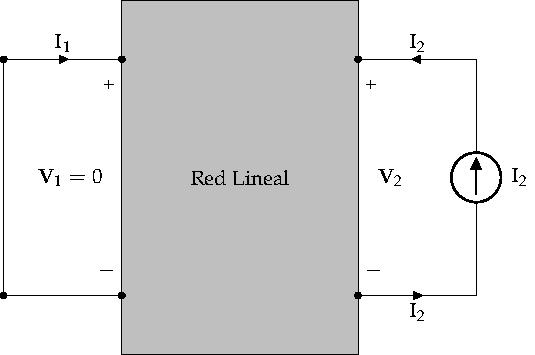
\includegraphics[height=4cm]{../figs/parametrosG_salida.pdf}
  \end{center}
\end{minipage}

\section{Impedancia de carga}

\begin{minipage}{0.5\textwidth}
  \begin{center}
    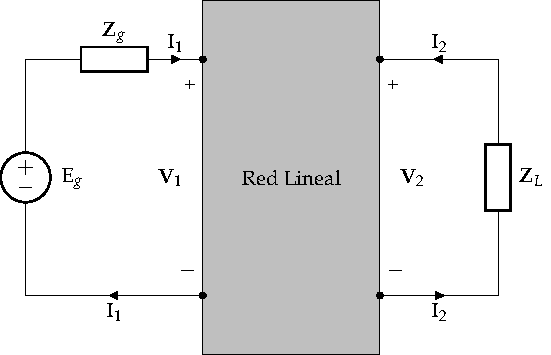
\includegraphics[height=4cm]{../figs/cuadripolo_cargado_fuente_tension.pdf}
  \end{center}
\end{minipage}
\begin{minipage}{0.5\textwidth}
  \begin{align*}
    \mathbf{U}_1 &= \mathbf{E}_g - \mathbf{Z}_g \cdot \mathbf{I}_1\\
    \mathbf{U}_2 &= - \mathbf{Z}_L \cdot \mathbf{I}_2\\
  \end{align*}
\end{minipage}

\vspace{1cm}

Para obtener la máxima potencia en la salida del cuadripolo, la impedancia de carga $\mathbf{Z}_L$ deberá ser igual al conjugado de la impedancia de salida del cuadripolo, $\mathbf{Z}_L = \mathbf{Z}^*_o$, definida como:

\[
  \mathbf{Z}_o = \left.\dfrac{\mathbf{U}_2}{\mathbf{I}_2}\right\rvert_{\mathbf{E}_g = 0}
\]

Esta impedancia puede calcularse con cualquiera de las familias de parámetros anteriores. Por ejemplo, con los parámetros impedancia tendremos las siguientes ecuaciones:

\begin{align*}
  \mathbf{U}_1 &= - \mathbf{Z}_g \cdot \mathbf{I}_1\\
  \mathbf{U}_1 &= \mathbf{z}_{11} \mathbf{I}_1 + \mathbf{z}_{12} \mathbf{I}_2\\
  \mathbf{U}_2 &= \mathbf{z}_{21} \mathbf{I}_1 + \mathbf{z}_{22} \mathbf{I}_2\\
\end{align*}

Sustituyendo la primera ecuación en la segunda, y ésta a su vez en la tercera obtenemos:

\begin{equation*}
  \mathbf{Z}_o = \mathbf{z}_{22} - \dfrac{\mathbf{z}_{12} \cdot \mathbf{z}_{21}}{\mathbf{Z}_g + \mathbf{z}_{11}}
\end{equation*}

\clearpage

\section{Ejemplo: red en T}

\begin{center}
  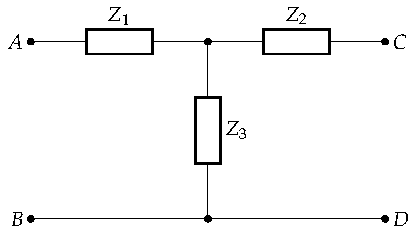
\includegraphics[height=4cm]{../figs/cuadripolo_T}
\end{center}

\begin{minipage}[t]{0.5\textwidth}
  \subsection*{Parámetros impedancia}

  \begin{align*}
    \mathbf{z}_{11} &= \mathbf{Z}_1 + \mathbf{Z}_3\\
    \mathbf{z}_{12} &= \mathbf{Z}_3\\
    \mathbf{z}_{21} &= \mathbf{Z}_3\\
    \mathbf{z}_{22} &= \mathbf{Z}_2 + \mathbf{Z}_3
  \end{align*}
\end{minipage}
\begin{minipage}[t]{0.5\textwidth}
  \subsection*{Parámetros admitancia}

    \begin{align*}
      \mathbf{y}_{11} &= \dfrac{\mathbf{Z}_2 + \mathbf{Z}_3}{\mathbf{Z}_1\mathbf{Z}_2 + \mathbf{Z}_1\mathbf{Z}_3 + \mathbf{Z}_2\mathbf{Z}_3}\\
      \mathbf{y}_{12} &= \dfrac{-\mathbf{Z}_3}{\mathbf{Z}_1\mathbf{Z}_2 + \mathbf{Z}_1\mathbf{Z}_3 + \mathbf{Z}_2\mathbf{Z}_3}\\
      \mathbf{y}_{21} &= \dfrac{- \mathbf{Z}_3}{\mathbf{Z}_1\mathbf{Z}_2 + \mathbf{Z}_1\mathbf{Z}_3 + \mathbf{Z}_2\mathbf{Z}_3}\\
      \mathbf{y}_{22} &= \dfrac{\mathbf{Z}_1 + \mathbf{Z}_3}{\mathbf{Z}_1\mathbf{Z}_2 + \mathbf{Z}_1\mathbf{Z}_3 + \mathbf{Z}_2\mathbf{Z}_3}
    \end{align*}
\end{minipage}

\vspace{1cm}

\begin{minipage}[t]{0.5\textwidth}
  \subsection*{Parámetros híbridos}

  \begin{align*}
    \mathbf{h}_{11} &= \dfrac{\mathbf{Z}_1\mathbf{Z}_2 + \mathbf{Z}_1\mathbf{Z}_3 + \mathbf{Z}_2\mathbf{Z}_3}{\mathbf{Z}_2 + \mathbf{Z}_3}\\
    \mathbf{h}_{12} &= \dfrac{\mathbf{Z}_3}{\mathbf{Z}_2 + \mathbf{Z}_3}\\
    \mathbf{h}_{21} &= \dfrac{- \mathbf{Z}_3}{\mathbf{Z}_2 + \mathbf{Z}_3}\\
    \mathbf{h}_{22} &= \dfrac{1}{\mathbf{Z}_2 + \mathbf{Z}_3}
  \end{align*}
\end{minipage}
\begin{minipage}[t]{0.5\textwidth}
  \subsection*{Parámetros híbridos inversos}

  \begin{align*}
    \mathbf{g}_{11} &= \dfrac{1}{\mathbf{Z}_1 + \mathbf{Z}_3}\\
    \mathbf{g}_{12} &= \dfrac{-\mathbf{Z}_3}{\mathbf{Z}_1 + \mathbf{Z}_3}\\
    \mathbf{g}_{21} &= \dfrac{\mathbf{Z}_3}{\mathbf{Z}_1 + \mathbf{Z}_3}\\
    \mathbf{g}_{22} &= \dfrac{\mathbf{Z}_1\mathbf{Z}_2 + \mathbf{Z}_1\mathbf{Z}_3 + \mathbf{Z}_2\mathbf{Z}_3}{\mathbf{Z}_1 + \mathbf{Z}_3}
  \end{align*}
\end{minipage}
\end{document}

%%% Local Variables:
%%% mode: latex
%%% ispell-local-dictionary: "castellano"
%%% End:
